%%%%%%%%%%%%%%%%%%%%%%%%%%%%%%%%%%%%%%%%%%%%%%%%%%%%%%%%%%%%%%%%%%%%%%%%%%%%%%%
% Copyright (C)  2015 Philipp Hacker
% Permission is granted to copy, distribute and/or modify this document
% under the terms of the GNU Free Documentation License, Version 1.3
% or any later version published by the Free Software Foundation;
% with no Invariant Sections, no Front-Cover Texts, and no Back-Cover Texts.
% A copy of the license should come with this file and/or can be obtained at
% http://www.gnu.org/licenses/fdl-1.3.html
%%%%%%%%%%%%%%%%%%%%%%%%%%%%%%%%%%%%%%%%%%%%%%%%%%%%%%%%%%%%%%%%%%%%%%%%%%%%%%%

\documentclass{beamer}
%\usetheme{UniGreifswald}
\usetheme{Warsaw}
\useoutertheme{infolines}

\beamertemplatenavigationsymbolsempty
\setbeamertemplate{footline}[page number]

\usepackage[ngerman]{babel}
\usepackage[T1]{fontenc}
\usepackage[utf8]{inputenc}

\usepackage[autostyle=true]{csquotes}
\usepackage[%
%			style=authortitle,%
			style=verbose,%
			autocite=footnote,%
			maxbibnames=15,%
			maxcitenames=15,%
			babel=hyphen,%
			hyperref=true,%
			abbreviate=false,%
			backend=bibtex,%
			mcite%
%			labelyear
]{biblatex}

\addbibresource{bibcontents/preamble.bib} % The filename of the bibliography
\addbibresource{bibcontents/master.bib} % The filename of the bibliography

\usepackage{mathtools}
\usepackage{graphicx}
\usepackage{units}
\usepackage{siunitx}
\usepackage{caption}
\usepackage{subcaption}
\captionsetup{labelformat=empty,labelsep=none}

\usepackage{tikz}
\usetikzlibrary{positioning}

\newcommand{\diff}{\text{d}}
\newcommand{\tenpo}[1]{\cdot 10^{#1}}
\newcommand{\ix}[1]{_\text{#1}}
\newcommand{\imag}{\mathbf{i}}
\newcommand{\fett}[1]{\textbf{#1}}



\newcommand{\stichpunkt}[1]{\begin{itemize} \item #1 \end{itemize}}
\newcommand{\stichpfeil}[1]{\begin{itemize} \item[$\Rightarrow$] #1 \end{itemize}}



\renewcommand*{\bibfont}{\scriptsize}
\renewcommand*{\footnotesize}{\fontsize{5}{5}}



\newcommand{\backupend}{\setcounter{framenumber}{\value{finalframe}}}
\newcommand{\backupbegin}{\newcounter{finalframe}%
	\setcounter{finalframe}{\value{framenumber}}}



\title{Kinetic\ Effects\ in\ RF\ Discharges}
\author[P. Hacker]{Philipp\ Hacker}
\date{08.12.2017}
\institute[Uni Greifswald]%
{%
	Mathematisch-Naturwissenschaftliche\ Fakultät\\%
	Institut\ für\ Physik\\%
  	Ernst-Moritz-Arndt-Universität\ Greifswald%
}

\begin{document}
%
% Title-Folie mit Betreuer/Gutachter:
	\begin{frame}
	    \tikz[overlay,remember picture]{ 
			\node[at=(current page.north west)] (source) {};
			\node[opacity = 0.08, below right= 0.168\paperheight and -0.335\paperheight of source] {
				
\includegraphics[height=0.85\paperheight]{Uni-Siegel.png}
				}
			}
		\maketitle%
		\centering%
		{\scriptsize Betreuer:\ Prof.\ Dr.\ R.\ Schneider}\\%
		{\scriptsize Gutachter:\ Prof.\ Dr.\ J.\ Meichsner}%
	\end{frame}
%	
% Folie mit Inhaltsverzeichnis:
	\frame{\tableofcontents}
%
% Motivations-Sektion:
	\section{Motivation}
%
% Kapazitiv gekoppelte RF-Plasmen:
		\begin{frame}{Kapazitive gekopplte RF-Plasmen}
			\begin{columns}
				\begin{column}{0.45\textwidth}
					\begin{block}{}
						\stichpunkt{Anwendung in Technologie-Industrie bei Sputter- und Ätzprozessen}%
						\stichpunkt{Energieverteilungen der Plasmaspezies besonders wichtig}%
						\stichpunkt{schnelle Anionen in CCRF-Entladungen}%
					\end{block}
				\end{column}
				\begin{column}{0.45\textwidth}
					\begin{figure}%
						\includegraphics[width=\textwidth]%
										{figures/circuitselfbias_1.png}%
						\caption{{\scriptsize%
								(Schema einer Entladung\footnotemark)}}%
					\end{figure}%
				\end{column}%
			\end{columns}%
			\footcitetext{Piel10}%
		\end{frame}%
	
		\begin{frame}{Experiment}%
			\begin{columns}
				\begin{column}{0.5\textwidth}
					\begin{figure}%
						\centering
						\includegraphics[width=1.0\textwidth]%
										{figures/SFB/neg_mg_one_only.png}%
						\caption*{{\scriptsize%
									(EVF negativer Ionen, Experiment\footnotemark)}}%
					\end{figure}%
				\end{column}
				\footcitetext{Matthias15}
				\begin{column}{0.45\textwidth}
					\begin{block}{}
						\stichpunkt{asymmetrische Niederdruckentladung in Sauerstoff\\%
									$\Rightarrow$ Self-Bias}
						\stichpunkt{hauptsächlich Produktion der O$^{-}$ durch diss. Anlagerung}
						\stichpunkt{Vermutung: Bildung negativer Ionen an der Kathodenoberfläche}
					\end{block}
				\end{column}
			\end{columns}
		\end{frame}%	
%
% Particle-in-Cell Simulation:
	\section{Particle-in-Cell Methode}
%
% Particle-in-Cell Simulation:
		\begin{frame}{Particle-in-Cell Methode}%
			\begin{figure}%
				\centering%
				\includegraphics[width=0.75\textwidth]%
								{figures/picscheme.pdf}
				\caption*{{\scriptsize%
							(PIC-Zyklus\footnotemark)}}
				\footcitetext{Matthias15}
				\addtocounter{footnote}{-1}
			\end{figure}
			\vspace{-1.0cm}
			\begin{block}{Stabilitätsbedingungen}
				\centering$%
				\Delta t\le\frac{\omega\ix{p,e}}{5},%
				\quad\quad\quad%
				\Delta r\le\frac{\lambda\ix{D,e}}{2}%
				$
			\end{block}	
		\end{frame}
%
% Boltzmann-Gleichung:
			\begin{frame}{Particle-in-Cell Methode}
				\begin{block}{Boltzmann-Gleichung}
					\raggedright%
					Lösen in jedem Schritt:
					\begin{align*}
						\frac{\partial f\ix{j}}{\partial t}+\vec{v}\cdot\nabla_{\vec{r}}\,f\ix{j}%
						+&\frac{q\ix{j}}{m\ix{j}}\vec{E}\cdot\nabla_{\vec{v}}\,f\ix{j}%
						=\left(\frac{\partial f\ix{j}}{\partial t}\right)\ix{Coll}%
						\onslide<2>{%
							\\&\Bigg\Downarrow%
							Linearisierung%
							\\%
							f\ix{j}(x,v,t+\Delta t)=%
								(1+\Delta& t\cdot I)(1+\Delta t\cdot D)f\ix{j}(x,v,t)%
						}
					\end{align*}
				\end{block}
				\onslide<2>{\begin{alertblock}{}%
					wenige Stöße und große freie Weglängen\\%
					$\Rightarrow$ kinetische Simulation notwendig%
				\end{alertblock}}
			\end{frame}
%		
% Vergleich mit 1D Simulationen:  
	\section{1D Simulation}
%
% Ergebnisse von 1D:
		\begin{frame}{1D Simulation}%
			\begin{columns}
				\begin{column}{0.6\textwidth}
					\begin{figure}
						\centering%
						\includegraphics[height=0.6\textheight]%
										{figures/SFB/5Pa_densities_zoom.png}
						\caption*{{\scriptsize%
								(Dichten einer Entladung bei~800~V$\ix{pp}$~%
								und~\SI{5}{\pascal}\footnotemark,\\
								Trennung der Anionen auf Oberflächen- und Volumenprozesse)}}%
					\end{figure}
				\end{column}
				\begin{column}{0.40\textwidth}
					\begin{block}{}
						\stichpunkt{Treiber bei $x=0$ (hier SIE), geerdete Elektrode gegenüber}
						\stichpunkt{experimenteller Wert für Injektions-Effizienz\\%
									$\eta=\frac{I(O^{-})}{I(O^{+}_{2})}=0,03$}
						 \stichpunkt{Anionen-EVF verschoben und Peak vor getriebener Elektrode}
					\end{block}
				\end{column}
				\footcitetext{Matthias17}%
				\addtocounter{footnote}{-1}
			\end{columns}
		\end{frame}%

%                   	
% Energieverteilungen:
		\begin{frame}{Dynamik negativer Ionen}%
			\begin{block}{}
				\stichpunkt{Beschleunigung/Reflexion in der Randschicht \&~%
							zusätzlicher Peak bei hohen Energien}
			\end{block}
			\begin{figure}
				\centering%
				\includegraphics[width=0.6\textwidth]%
								{figures/SFB/5Pa_400V_energy_sims_top.png}
				\caption*{{\scriptsize%
							(EVF der $O^{-}$ von der Oberfläche; Entladung bei~800~V$\ix{pp}$~%
							und~\SI{5}{\pascal}\footnotemark)}}
			\end{figure}%
			\vspace*{-0.75cm}
			\footcitetext{Matthias17}%
			\addtocounter{footnote}{-1}
		\end{frame}%
%	
		\begin{frame}{Dynamik negativer Ionen}%
			\begin{figure}
				\centering%
				\includegraphics[width=0.6\textwidth]%
								{figures/SFB/elastic_coll_compose.png}
			\end{figure}%
			\vspace*{-0.5cm}
			\begin{block}{}{\scriptsize%
				elastische Stöße der $O^{-}$ ohne (links) und mit SIE (rechts, $\eta=0,03$, getrennte Anionenspezies)\footnotemark}
			\end{block}
			\footcitetext{Matthias17}%
			\addtocounter{footnote}{-1}
		\end{frame}%
%	
		\begin{frame}{Dynamik negativer Ionen}%
			\begin{columns}
				\begin{column}{0.5\textwidth}
					\begin{figure}
						\centering%
						\includegraphics[height=0.75\textheight]%
										{figures/SFB/time_solo.png}
					\end{figure}%
				\end{column}
				\begin{column}{0.5\textwidth}
					\begin{block}{}
						\stichpunkt{Dichtefront in Randschicht durch langsame Anionen}
						\stichpunkt{Eintrittsenergie $\sim$\SI{50}{\electronvolt}}
						\stichpunkt{Anion verbleibt 4-5 RF-Zyklen in der Randschicht}
					\end{block}
					\begin{alertblock}{}
						\stichpfeil{niederenergetische Peaks vor getriebener Elektrode}
					\end{alertblock}
					\begin{flushleft}
						{\scriptsize%
							(Phase der EVF von Oberflächen-Anionen bei $U\ix{rf}=0$, Entladung bei 1600~V$\ix{pp}$ und \SI{5}{\pascal}\footnotemark)}
					\end{flushleft}
				\end{column}
				\footcitetext{Matthias17}%
				\addtocounter{footnote}{-1}
			\end{columns}
		\end{frame}%
%	
		\begin{frame}{Simulationsergebnisse}%
			\begin{columns}
				\begin{column}{0.4\textwidth}
					\begin{block}{}
						\stichpunkt{qualitative Übereinstimmung mit Experiment}
						\stichpunkt{niederenergetischer Peak durch intrinsiche Symmetrie}
					\end{block}
					\begin{alertblock}{}
						\stichpfeil{schnelle Anionen treffen nicht auf gegenüberliegende Elektrode}
					\end{alertblock}
				\end{column}
				\begin{column}{0.6\textwidth}
					\vspace*{-0.5cm}
					\begin{figure}
						\centering%
						\includegraphics[height=0.55\textheight]%
										{figures/SFB/power_energy_cuts.png}
					\end{figure}%
					\vspace*{-0.7cm}
					\begin{flushright}
						{\scriptsize\flushright%
							(Anionen-EVF versch. Spannungen vor Randschicht der geerdeten Elektrode; bei \SI{5}{\pascal} mit $\eta=0,03$~\footnotemark)}	
					\end{flushright}
				\end{column}
				\footcitetext{Matthias17}%
				\addtocounter{footnote}{-1}
			\end{columns}
		\end{frame}%
%
		\begin{frame}{Experiment-Ergebnisse}%
			\addtocounter{footnote}{-2}
			\begin{columns}
				\begin{column}{0.5\textwidth}
					\begin{figure}
						\centering%
						\includegraphics[width=\textwidth]%
										{figures/SFB/neg_mg_one_only.png}
						\caption*{{\scriptsize%
									(Anionen-EVF an geerdeter Elektrode, Experiment-Ergebnisse einer $MgO$-Elektrode~\footnotemark)}}
					\end{figure}%
				\end{column}
				\footcitetext{Matthias15}
				\begin{column}{0.5\textwidth}
					\begin{block}{}
						\stichpunkt{keine zusätzliche niederenergetische Struktur}
						\stichpfeil{durch invasive Messungen im Experiment entfernt}
						\stichpunkt{Steuerung über Generator-Leistung, indirekt die Elektrodenspannung}
						\stichpunkt{weitere hochenergetische Struktur in Anionen-EVF}
					\end{block}
				\end{column}
			\end{columns}
		\end{frame}%
%	
		\begin{frame}{Simulationen in 2D}%
			\begin{columns}
				\begin{column}{0.5\textwidth}
					\begin{block}{}
						\stichpunkt{}
					\end{block}
				\end{column}
				\begin{column}{0.5\textwidth}
				\end{column}
			\end{columns}
		\end{frame}

%
% Ausblick:
	\section{Ausblick}
%
		\begin{frame}{Fazit \& Ausblick}
			\begin{columns}
				\begin{column}{0.46\textwidth}
					\begin{alertblock}{Zusammenfassung}%
						\stichpunkt{}%
					\end{alertblock}
				\end{column}
				\begin{column}{0.46\textwidth}
					\begin{exampleblock}{Ausblick}%
						\stichpunkt{}%
					\end{exampleblock}
				\end{column}
			\end{columns}
		\end{frame}
%
		\begin{frame}
		\end{frame}

% Referenzen:
		\begin{frame}{Referenzen}
			\begin{columns}
				\begin{column}{0.1\textwidth}
				\end{column}
				\begin{column}{0.75\textwidth}
					\printbibliography
				\end{column}
			\end{columns}
		\end{frame}























%%%%%%%%%%%%%%%%%%%%%%%%%%%%%%%%%%%%%%%%%%%%%%%%%%%%%%%%%%%%%%%%%%%%%%%%%%%%%%%
%%%%%%%%%%%%%%%%%%%%%%%%%%%%%%%%%%%%%%%%%%%%%%%%%%%%%%%%%%%%%%%%%%%%%%%%%%%%%%%
%%%%%%%%%%%%%%%%%%%%%%%%%%%%%%%%%%%%%%%%%%%%%%%%%%%%%%%%%%%%%%%%%%%%%%%%%%%%%%%
%%%%%%%%%%%%%%%%%%%%%%%    REST REST REST REST REST   %%%%%%%%%%%%%%%%%%%%%%%%%
%%%%%%%%%%%%%%%%%%%%%%%%%%%%%%%%%%%%%%%%%%%%%%%%%%%%%%%%%%%%%%%%%%%%%%%%%%%%%%%
%%%%%%%%%%%%%%%%%%%%%%%%%%%%%%%%%%%%%%%%%%%%%%%%%%%%%%%%%%%%%%%%%%%%%%%%%%%%%%%
%%%%%%%%%%%%%%%%%%%%%%%%%%%%%%%%%%%%%%%%%%%%%%%%%%%%%%%%%%%%%%%%%%%%%%%%%%%%%%%

	\appendix
	\backupbegin
	
		\begin{frame}
		\end{frame}

		\begin{frame}{Randschicht}%
			\begin{columns}
				\begin{column}{0.45\textwidth}%
					\addtocounter{footnote}{-1}
				 	\begin{figure}%
						\includegraphics[width=\textwidth]%
										{figures/sheath_piel.png}%
						\caption{{\scriptsize\raggedright%
								  (Schema einer Randschicht\footnotemark)}}%
					\end{figure}%
				\end{column}%
				\footcitetext{Piel10}
				\begin{column}{0.45\textwidth}%
					\begin{block}{}%
						\stichpunkt{negative Aufladung der Wände durch schnellere Elektronen\newline%
									$\rightarrow$Self-Bias}%
						\stichpunkt{Ionen werden auf Bohm-Geschwindigkeit beschleunigt\newline%
									$v\ix{i,B}=\sqrt{\frac{k\ix{B}T\ix{e}}{m\ix{i}}}$}%
						\stichpunkt{Asymmetrie der getriebenen/geerden Elektroden}%
					\end{block}%
				\end{column}%
			\end{columns}%
		\end{frame}%

		\begin{frame}{Oberflächen- und Stoßprozesse}%
			\begin{figure}%
				\centering%
				\includegraphics[height=0.8\textheight]%
								{figures/xsections_selection.pdf}%
			\end{figure}%
		\end{frame}%

		\begin{frame}{Experiment}%
			\begin{columns}%
				\begin{column}{0.48\textwidth}%
					\begin{block}{}%
						\stichpunkt{große Asymmetrie zwischen geerdeter~%
									Kammer und CCRF-Elektrode}%
						\stichpunkt{niedrige Gasflüsse und -drücke~%
									($\le$\SI{5}{sc\centi\meter}, \SI{15}{\pascal})}%
						\stichpunkt{Elektrodenabstand~%
									$\sim$\SI{5}{\centi\meter}}%
					\end{block}%	
				\end{column}%
				\begin{column}{0.48\textwidth}%
					\begin{figure}%
						\centering
						\includegraphics[width=\textwidth]%
										{figures/chamber_exp.pdf}%
						\caption{{\scriptsize%
								(Experiment-Reaktor, Draufsicht\footnotemark)}}%
					\end{figure}%	
				\end{column}%
				\footcitetext{Matthias15}
			\end{columns}%
		\end{frame}%

		\begin{frame}{Experiment-Ergebnisse}%
			\addtocounter{footnote}{-1}
			\begin{figure}%
				\includegraphics[width=0.75\textwidth]%
								{figures/neg_mg.png}%
				\caption*{{\scriptsize%
						(Anionen-EVF an geerdeter Elektrode, Experiment-Ergebnisse %
						einer $MgO$-Elektrode~\footnotemark)}}
			\end{figure}%
			\footcitetext{Matthias15}
		\end{frame}%
	
		\begin{frame}{Saha-Langmuir}%
			\addtocounter{footnote}{-1}
			\begin{figure}%
				\centering%
				\includegraphics[height=0.3\textheight]%
								{figures/saha_langmuir.pdf}%
				\caption*{{\scriptsize%
							(Schema der Oberflächenprozesse negativer %
							und positiver Ionen\footnotemark)}}
			\end{figure}%
			\footcitetext{Matthias15}
			\begin{block}{Saha-Langmuir Gleichung:}\centering$%
					\alpha^{-}(X^{-})=\frac{(1-r^{-})}{(1-r)}\cdot%
						\frac{w^{-}}{w}\exp\left(%
						\frac{-\overline{\Phi}_{-}+e\sqrt{eV\ix{ext}}+A(X)}{k\ix{B}T}\right)%
					$%
			\end{block}
		\end{frame}%

		\begin{frame}{1D Simulation}
			\begin{figure}
				\begin{subfigure}{0.49\textwidth}
					\begin{overprint}
						\onslide<1>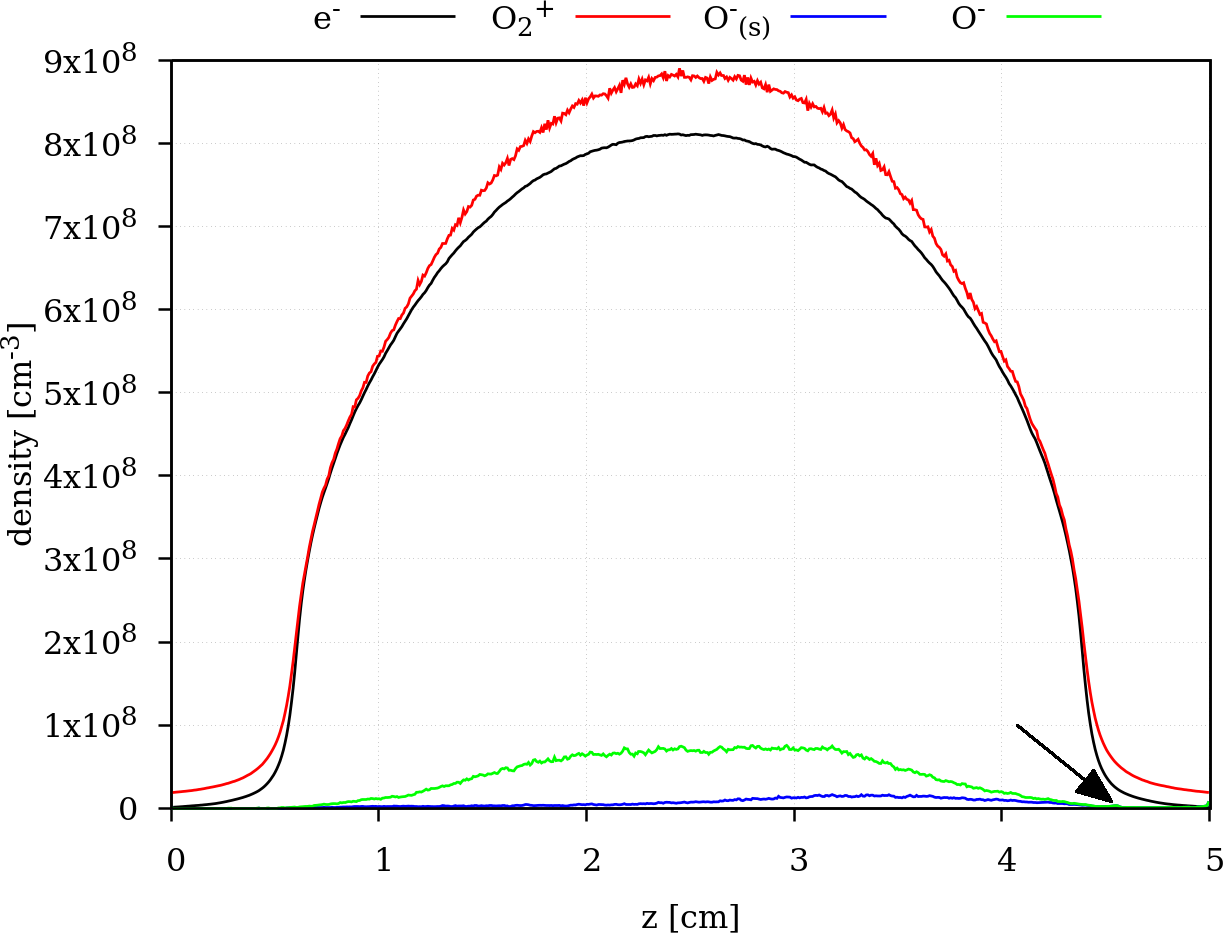
\includegraphics[width=0.9\textwidth]
										{figures/results/1D/densities.png}
						\onslide<2>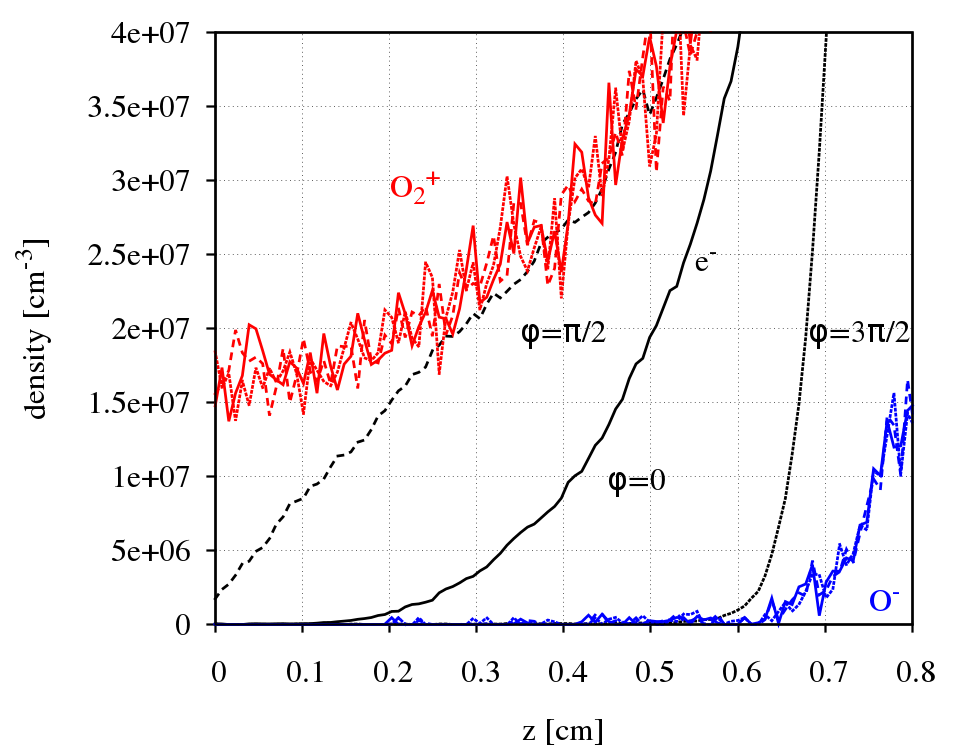
\includegraphics[width=0.9\textwidth]
										{figures/results/1D/prs_ne_dens.png}
					\end{overprint}
				\end{subfigure}
				\begin{subfigure}{0.49\textwidth}
					\begin{overprint}
						\onslide<1>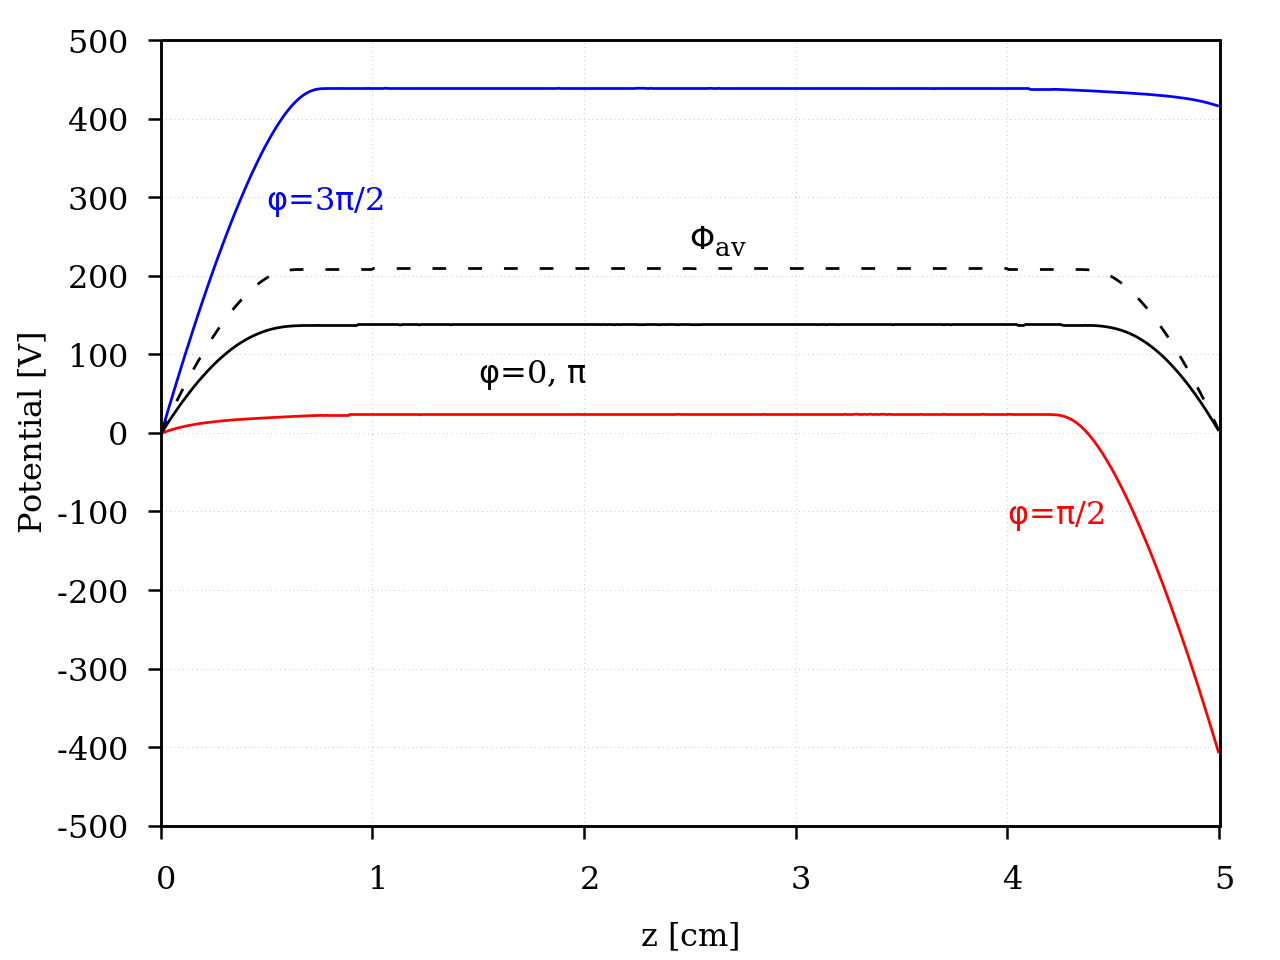
\includegraphics[width=0.9\textwidth]
											{figures/results/1D/potential.png}
						\onslide<2>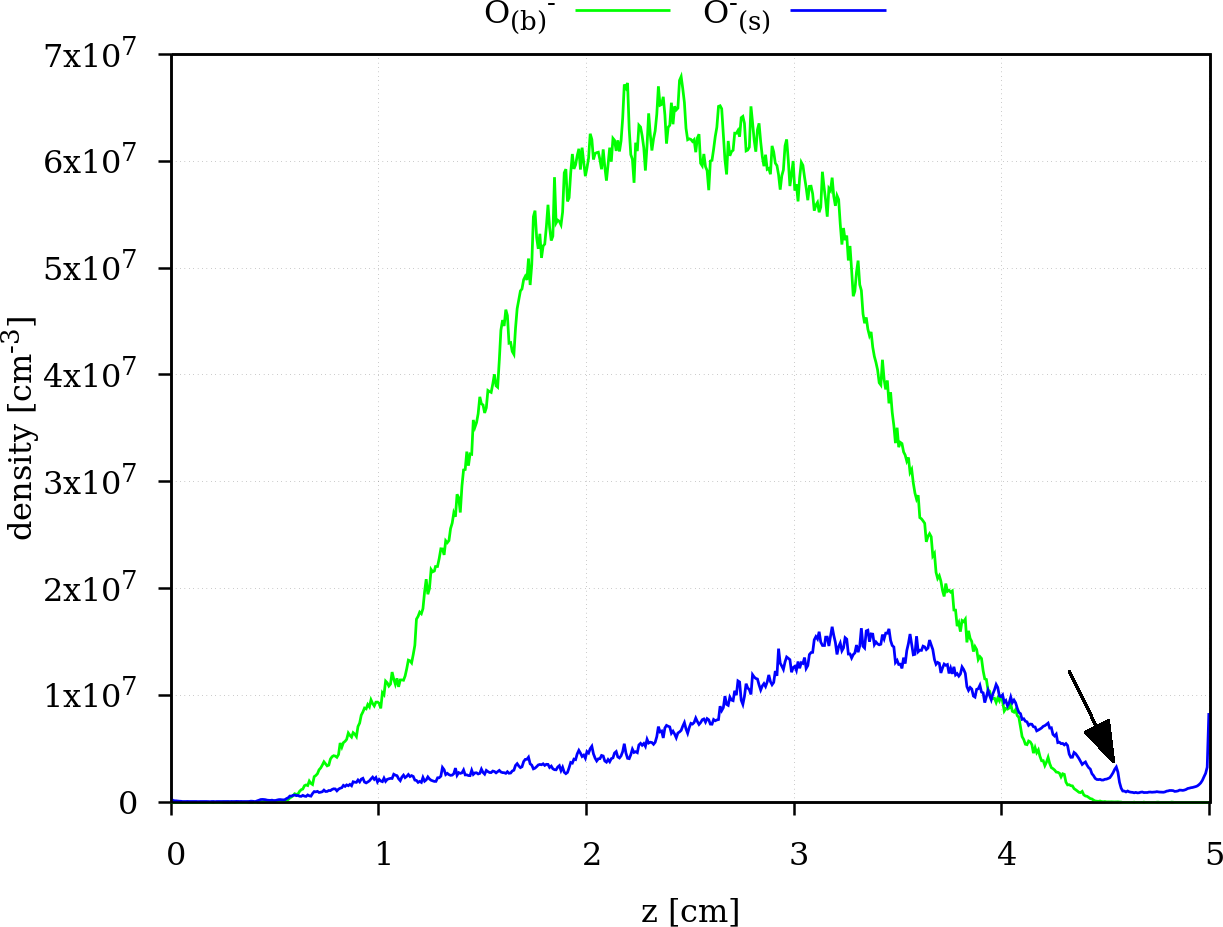
\includegraphics[width=0.9\textwidth]
											{figures/results/1D/densities_Omin.png}
					\end{overprint}
				\end{subfigure}
				\caption{{\scriptsize%
							(1D Simulationen; Entladung bei~
						  	\SI{5}{\pascal} und \SI{400}{\volt})}}
			\end{figure}
			\begin{block}{}
					\stichpunkt{Dichte und phasenaufgelöstes Potential in 1D mit~%
								Injektion negativer Ionen von der Kathode}%
					\stichpfeil{$\eta = \frac{I(O^{-})}{I(O^{+}_{2})} = 0,03$}
			\end{block}
		\end{frame}

		\begin{frame}{Dynamik negativer Ionen}%
			\begin{figure}%
				\centering%
				\begin{subfigure}{0.5\textwidth}%
					\includegraphics[width=\textwidth]%
									{figures/results/1D/snix_edf.png}%
					\caption*{{\scriptsize%
								(Energieverteilung der negativen Ionen von der Oberfläche)}}%
				\end{subfigure}%
				\begin{subfigure}{0.5\textwidth}%
					\begin{overprint}%
						\onslide<1>\includegraphics[width=0.95\textwidth]%
													{figures/results/1D/snix_close_edf.png}%
						\caption*{{\scriptsize%
									(Anodenbereich der EVF von O$^{-}$)}}%
						\onslide<2>\includegraphics[width=0.95\textwidth]%
													{figures/results/1D/snix_surface_edf.png}%
						\caption*{{\scriptsize%
									(Surfaceplot der O$^{-}$ EVF)}}%
						\onslide<3>\includegraphics[width=0.95\textwidth]%
														{figures/results/1D/ix_edf.png}%
						\caption*{{\scriptsize%
									(EVF der O$^{+}_{2}$ Ionen)}}%
						\onslide<4>\includegraphics[width=0.95\textwidth]%
													{figures/results/1D/ex_edf.png}%
						\caption*{{\scriptsize%
									(EVF der Elektronen)}}%
					\end{overprint}%
				\end{subfigure}%
			\end{figure}%
		\end{frame}%

		\begin{frame}{Dynamik negativer Ionen}%
			\begin{figure}%
				\centering%
				\includegraphics[height=0.75\textheight]%
								{figures/results/1D/snix_allpi_edf.png}%
				\caption*{{\scriptsize%
						(Phasenaufgelöster Anodenbereich, Energieverteilung der $O^{-}$)}}%
			\end{figure}%
		\end{frame}%
          	 	            	
		\begin{frame}{Simulationen in 2D}
			\begin{exampleblock}{}
					\stichpunkt{Annahme einer zylinder-symmetrische Entladung um Mitte %
								der Elektrode}
					\stichpunkt{jetzt: verschiedene Kombinationen von Randbedingungen,\linebreak%
								zBsp. Dielektrika}
					\stichpunkt{viel größerer numerischer Aufwand}
			\end{exampleblock}
			\begin{figure}%
				\centering%
				\begin{subfigure}{0.47\textwidth}
					\centering
					\includegraphics[height=0.35\textheight]%
						{figures/domain_slice.png}%
				\end{subfigure}
				\begin{subfigure}{0.47\textwidth}
					\centering
					\includegraphics[height=0.35\textheight]%
						{figures/radial_cylinder.png}%
					\end{subfigure}
			\end{figure}%
		\end{frame} 

		\begin{frame}{Vergleich mit 1D}%
			\begin{figure}%
				\begin{subfigure}{0.48\textwidth}%
					\begin{overprint}
						\centering%
						\onslide<1>\includegraphics[width=0.85\textwidth]%
							{figures/results/2D/compare/45365_dens.png}%
						\onslide<2>\includegraphics[width=0.85\textwidth]%
							{figures/results/2D/compare/onedtwod_45431_denscompare.png}%
					\end{overprint}
				\end{subfigure}
				\begin{subfigure}{0.48\textwidth}%
					\begin{overprint}
						\centering%
						\onslide<1>\includegraphics[width=0.85\textwidth]%
							{figures/results/2D/compare/45365prs_pot.png}%
						\onslide<2>\includegraphics[width=0.85\textwidth]%
							{figures/results/2D/compare/onedtwod_45431_phicompare.png}%
					\end{overprint}
				\end{subfigure}%
				\caption*{{\scriptsize%
						   (Dichten und Potentiale bei \SI{5}{\pascal} und 400~V$\ix{pp}$~%
				  			im Vergleich)}}%
			\end{figure}%
			\begin{alertblock}{}
				$\Rightarrow$ globales Flussgleichgewicht verändert Plasma %
				um den Gesamtstrom in die Randschichten anzugleichen
			\end{alertblock}
		\end{frame}%

		\begin{frame}{2D Profile}%
			\begin{figure}%
				\centering%
				\vspace*{0.7cm}
				\includegraphics[height=0.8\textheight]%
								{figures/results/2D/compare/twod_alldensphi_45431.png}%
			\end{figure}%
		\end{frame}%
	
		\begin{frame}{Asymmetrische Ranbedingungen}%
			\begin{columns}%
				\begin{column}{0.45\textwidth}%
					\begin{figure}%
						\centering%
						\begin{overprint}%
							\onslide<1>\includegraphics[width=0.85\textwidth]%
											  			{figures/results/2D/44332/phi.png}%
							\caption*{{\scriptsize%
										(Potential, \SI{5}{\pascal}, \SI{500}{\volt},\linebreak%
										 $U_{sb}=$\SI{-400}{\volt})}}%
							 \onslide<2>\includegraphics[width=0.85\textwidth]%
														{figures/results/2D/44332/i_dens.png}%
							\caption*{{\scriptsize%
										(Ionendichte, \SI{5}{\pascal},\linebreak%
										 \SI{400}{\volt}, $U_{sb}=$\SI{-500}{\volt})}}%
							\onslide<3>\includegraphics[width=0.85\textwidth]%
														{figures/results/2D/44332/i_velz.png}%
							\caption*{{\scriptsize%
										(axiale Ionengeschwindigkeit,\linebreak%
								 		\SI{5}{\pascal}, \SI{400}{\volt}, %
										 $U_{sb}=$\SI{-500}{\volt})}}%
						\end{overprint}%
					\end{figure}%
				\end{column}%
				\begin{column}{0.45\textwidth}
					\begin{block}{}%
						\stichpunkt{linke Elektrode getrieben, restliche %
									Randbedingungen sind geerdet}
						\stichpunkt{Asymmetrie des Bulk und der Randschichten}
						\stichpunkt{größere Beschleunigung bei kleinerer Randschicht}%
					\end{block}%
				\end{column}%
			\end{columns}%
		\end{frame}%

		\begin{frame}{Asymmetrische Ranbedingungen}%
			\begin{columns}%
				\begin{column}{0.45\textwidth}
					\begin{block}{}%
						\stichpunkt{beide Elektroden getrieben, obere/linke %
									Bereiche geerdet und rechts `floatet'\linebreak%
									$\Rightarrow$ offene Randbedingung}
						\stichpunkt{sehr viel höheres Plasmapotential}
						\stichpunkt{ähnliche Randschichten, größer als zuvor geringere Geschwindigkeiten}
					\end{block}%
				\end{column}%
				\begin{column}{0.45\textwidth}%
					\begin{figure}%
						\centering%
						\begin{overprint}%
							\onslide<1>\includegraphics[width=0.85\textwidth]%
											  			{figures/results/2D/44426/phi.png}%
							\caption*{{\scriptsize%
										(Potential, \SI{5}{\pascal}, \SI{400}{\volt},\linebreak%
										 $U_{sb}=$\SI{-400}{\volt})}}%
							 \onslide<2>\includegraphics[width=0.85\textwidth]%
														{figures/results/2D/44426/i_dens.png}%
							\caption*{{\scriptsize%
										(Ionendichte, \SI{5}{\pascal},\linebreak%
										 \SI{400}{\volt}, $U_{sb}=$\SI{-400}{\volt})}}%
							\onslide<3>\includegraphics[width=0.85\textwidth]%
														{figures/results/2D/44426/i_velz.png}%
							\caption*{{\scriptsize%
										(axiale Ionengeschwindigkeit,\linebreak%
										 \SI{5}{\pascal}, \SI{400}{\volt}, %
										 $U_{sb}=$\SI{-400}{\volt})}}%
						\end{overprint}%
					\end{figure}%
				\end{column}%
			\end{columns}%
		\end{frame}%

		\begin{frame}{Einfluss des Self-Bias}%
			\begin{columns}%
				\begin{column}{0.45\textwidth}%
						\begin{alertblock}{Erkenntnis}%
							Die negativen Ionen treffen auf die Anode mit hoher kinetischer %
							Energie aufgrund der zusätzlichen Beschleunigung in der Randschicht durch den Self-Bias.
						\end{alertblock}
					\end{column}%
					\begin{column}{0.45\textwidth}%
						\begin{figure}%
							\includegraphics[height=0.55\textheight]%
											{figures/results/2D/SFB/ni_distz.png}%
							\caption*{{\scriptsize%
								(axiale Ionenenergieverteilung,\linebreak%
								\SI{6}{\pascal}, \SI{400}{\volt} und $U_{sb}=$\SI{-200}{\volt})}}%
						\end{figure}%
					\end{column}%
				\end{columns}%
			\end{frame}%

			\begin{frame}{Einfluss des Self-Bias}%
				\begin{columns}%
					\begin{column}{0.45\textwidth}%
						\begin{alertblock}{}%
							\stichpunkt{stoßbehaftete Schicht $\Rightarrow$ kalte Ionen im Bulk}%
							\stichpunkt{Asymmetrie und Self-Bias notwendig zur Beschreibung der Effekte}%
						\end{alertblock}
				\end{column}%
				\begin{column}{0.45\textwidth}%
					\begin{figure}
						\includegraphics[height=0.5\textheight]%
										{figures/results/2D/SFB/ni_cut.png}%
						\caption*{{\scriptsize%
							(Ionenenergieverteilung an der Anode,\linebreak%
							\SI{6}{\pascal}, \SI{400}{\volt})}}%
					\end{figure}%
				\end{column}%
			\end{columns}%
		\end{frame}%

	\backupend

\end{document}
